\documentclass{homework}
\usepackage{float}
\usepackage[dvipsnames]{xcolor}
\usepackage{tikz}

\title{Tarea 2}
\date{2019-09-06}
\gdate{2do Semestre 2019}
\author{Nicholas Mc-Donnell}
\course{Variable Compleja - MAT2705}

\begin{document}
\maketitle
\pagenumbering{roman}
\newpage
\tableofcontents
\newpage
\pagenumbering{arabic}
\begin{prob}
    Demuestre que toda transformación de Möbius no constante puede representarse como
    \[\frac{az+b}{cz+d}\quad\text{con }ad-bc=1\]
\end{prob}

\begin{sol}
    Sea \(f\) una transformación de Möbius, entonces existen \(a,b,c,d\in\set{C}\) tal que \(f(z)=\frac{az+b}{cz+d}\), luego sea \(e^2=ad-bc\), se reescribe \(f(z)=\frac{a/ez+b/e}{c/ez+d/e}\), y se nota que con eso se tiene lo pedido.
\end{sol}

\begin{prob}
    Encuentre una transformación de Möbius que lleva \(1+i\) a \(0\), \(2\) a \(\infty\) y \(0\) a \(i-1\), y encuentre la imágen de \(\{\abs{z-1}<1\}\) bajo esta transformación.
\end{prob}

\begin{sol}
    Se nota que usando la primera y la segunda condición se tiene la siguiente transformación:
    \begin{equation*}
        k\cdot\frac{z-(1+i)}{z-2}
    \end{equation*}
    Agregando la tercera, se llega a que \(k=2i\), por lo que la transformación \(\frac{2iz+(2-2i)}{z-2}\) da lo pedido.\\
    Para ver la imágen de la transformación por conexidad es suficiente ver tres puntos en el borde la región, estos son \(1+i,2\) y \(0\), con ellos se nota que nos dan la siguiente región:
    \begin{figure}[H]
        \centering
        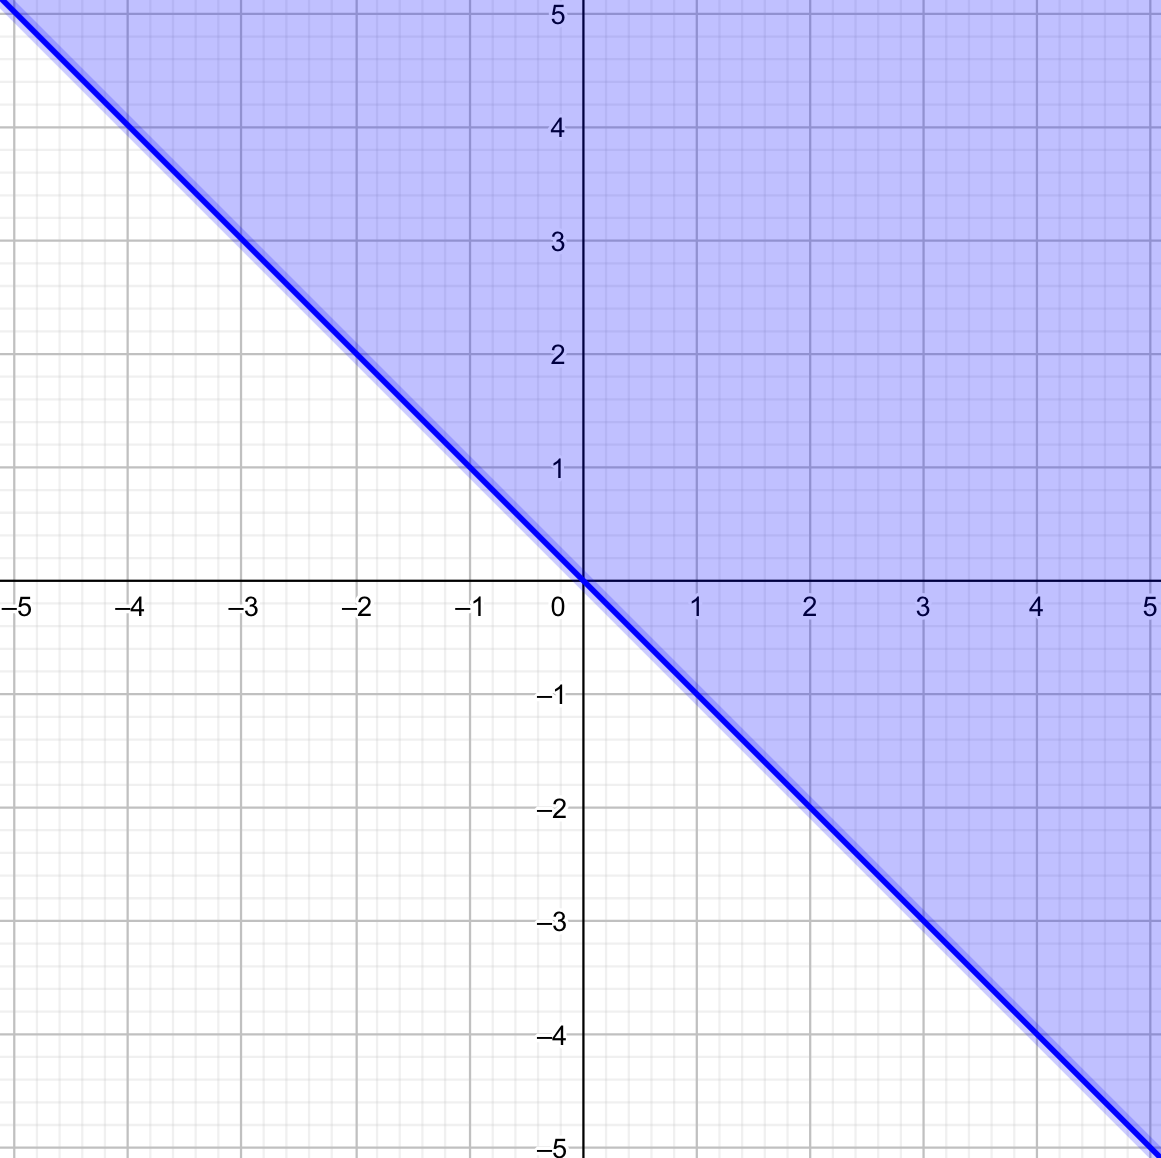
\includegraphics[width=6cm, height=6cm]{geogebra-export.png}
        \caption{Imagén de la transformación}
    \end{figure}
\end{sol}

\begin{prob}
    \begin{enumerate}[label=(\alph*)]
        \item Demuestre que las siguientes funciones son armónicas y determine su conjugado armónico en \(D\).
        \begin{enumerate}[label=(\roman*)]
            \item \(u(x,y)=\exp(x)\sin y\) en \(D=\set{C}\);
            \item \(u(x,y)=\sinh x\cos y\) en \(D=\set{C}\);
            \item \(u(x,y)=\frac{y}{x^2+y^2}\) en \(D=\set{C}\setminus(-\infty,0]\).
        \end{enumerate}
        \item Se define \(u(z)=\Im(z^{-2})\) para \(z\neq0\) y \(u(0)=0\).
        \begin{enumerate}[label=(\roman*)]
            \item Demuestre que todas las derivadas parciales de \(u\) existen en todo \(\set{C}\).
            \item Demuestre que \(\Delta u=0\).
            \item Demuestre que \(\frac{\partial^2u}{\partial x\partial y}\) no existe en \((0,0)\).
            \item Demuestre que \(u\) no posee conjugado armónico en \(\set{C}\).
        \end{enumerate}
    \end{enumerate}
\end{prob}

\begin{sol}
    \begin{enumerate}[label=(\alph*)]
        \item \begin{enumerate}[label=(\roman*)]
            \item Se ve que \(\frac{\partial^2 u}{\partial x^2}=\exp(x)\sin y\) y que \(\frac{\partial^2 u}{\partial y^2}=-\exp(x)\sin y\), por lo que \(\Delta u=0\). Usando las condiciones de Cauchy-Riemann se tiene lo siguiente:
            \begin{align*}
                \frac{\partial u}{\partial x}&=\frac{\partial v}{\partial y}=\exp(x)\sin y\\
                -\frac{\partial u}{\partial y}&=\frac{\partial v}{\partial x}=-\exp(x)\cos y
            \end{align*}
            Esto se resuelve integrando correspondientemente y viendo las constantes, y se llega a que \(v(x,y)=-\exp(x)\cos y+C\).
            \item Se ve que \(\frac{\partial^2 u}{\partial x^2}=\sinh x\cos y\) y que \(\frac{\partial^2 u}{\partial y^2}=-\sinh x\cos y\), por lo que \(\Delta u=0\). Usando las condiciones de Cauchy-Riemann se tiene lo siguiente:
            \begin{align*}
                \frac{\partial u}{\partial x}&=\frac{\partial v}{\partial y}=\cosh x\cos y\\
                -\frac{\partial u}{\partial y}&=\frac{\partial v}{\partial x}=\sinh x\sin y
            \end{align*}
            Esto se resuelve integrando correspondientemente y viendo las constantes, y se llega a que \(v(x,y)=\cosh x\sin y+C\).
            \item Se ve que \(\frac{\partial^2 u}{\partial x^2}=-\frac{2 y (y^2 - 3 x^2)}{(y^2 + x^2)^3}\) y que \(\frac{\partial^2 u}{\partial y^2}=\frac{2 y (y^2 - 3 x^2)}{(x^2 + y^2)^3}\), por lo que \(\Delta u=0\). Usando las condiciones de Cauchy-Riemann se tiene lo siguiente:
            \begin{align*}
                \frac{\partial u}{\partial x}&=\frac{\partial v}{\partial y}=-\frac{2yx}{(x^2+y^2)^2}\\
                -\frac{\partial u}{\partial y}&=\frac{\partial v}{\partial x}=-\frac{x^2-y^2}{(x^2+y^2)^2}
            \end{align*}
            Esto se resuelve integrando correspondientemente y viendo las constantes, y se llega a que \(v(x,y)=\frac{x}{x^2+y^2}+C\).
        \end{enumerate}
        \item Se nota que \(u(x,y)=-\frac{2xy}{(x^2+y^2)^2}\) y que \(u(0,0)=0\), lo cual es simétrico entre \(x\) e \(y\) (i.e. \(u(x,y)=u(y,x)\))
        \begin{enumerate}[label=(\roman*)]
            \item Para \(x,y\neq0\) es claro que existen, por lo que se ven los siguientes límites:
            \begin{equation*}
                \lim_{\Delta x\rightarrow 0}\frac{u(\Delta x,0)-u(0,0)}{\Delta x}=\lim_{\Delta x\rightarrow 0}\frac{0-0}{\Delta x}=0
            \end{equation*}
            Con lo que se tiene que existe \(\partial_x u\) en todo \(\set{C}\), luego por simetría se tiene que \(\partial_y x\) existe en todo \(\set{C}\).
            \item  Se calculan las segundas derivadas en todo punto (excepto \((0,0)\))
            \begin{align*}
                \frac{\partial^2 u}{\partial x^2}=\frac{\partial}{\partial x}\paren{\frac{-2 y (-3 x^2 + y^2)}{(x^2 + y^2)^3}}=\frac{24 x y (y^2 - x^2)}{(x^2 + y^2)^4}\\
                \frac{\partial^2 u}{\partial y^2}=\frac{\partial}{\partial y}\paren{\frac{-2 x (-3 y^2 + x^2)}{(x^2 + y^2)^3}}=\frac{24 x y (x^2 - y^2)}{(x^2 + y^2)^4}
            \end{align*}
            Por lo que claramente \(\Delta u=0\), ahora para el \((0,0)\), se ven los límites por definición:
            \begin{equation*}
                \lim_{\Delta x\rightarrow 0}\frac{\partial_x(\Delta x, 0)-\partial_x u(0, 0)}{\Delta x}=\lim_{\Delta x\rightarrow 0}\frac{0-0}{\Delta x}=0
            \end{equation*}
            Y de nuevo por simetría se tiene que \(\partial^2_x u(0,0)=\partial^2_y u(0,0)=0\), por lo que \(\Delta u=0\) para todo \(z\in\set{C}\)
            \item Se ve el siguiente límite:
            \begin{equation*}
                \lim_{\Delta x\rightarrow 0}\frac{\partial_y(\Delta x, 0)-\partial_y(0,0)}{\Delta x}=\lim_{\Delta x\rightarrow 0}\frac{\frac{-2\Delta x^3}{\Delta x^6}-0}{\Delta x}=\lim_{\Delta x\rightarrow 0}\frac{-2}{\Delta x^4}
            \end{equation*}
            Claramente el límite no existe, por lo que \(u\) no es \(C^2\)
            \item Se asume que existe \(v\) conjugado armónico de \(u\), luego \(f(z)=u+iv\) es analítica, por lo que \(f\in\mathcal{C}^\infty\), por lo que \(u\in\mathcal{C}^\infty\), pero \(\partial_xy u(0,0)\) no existe. Por lo que no existe \(v\) conjugado armónico de \(u\).
        \end{enumerate}
    \end{enumerate}
\end{sol}

\begin{prob}
    Sea \(n\in\set{N}\) y \(\lambda=\rho_0\exp(i\varphi_0)\). Encuentre el módulo máximo de \(z^n+\lambda\) en \(\{\abs{z}\leq r\}\).
\end{prob}

\begin{sol}
    Es claro que \(\abs{z^n+\lambda}\leq r^n+\abs{\rho_0}\), sea \(z=r\exp(i\varphi/n)\), se nota que \(\abs{z}=r\), luego \(\abs{z^n+\lambda}=r^n+\abs{\rho_0}\), por lo que se tiene el máximo.
\end{sol}

\begin{prob}
    Considere las curvas \(C_R^\delta=\{R\exp(\theta):\theta\in[\delta,\pi-\delta]\},C_R^+=\{z:\abs{z}=R,\Im(z)>0\}.C_R^-=\{z:\abs{z}=R,\Im(z)<0\}\) y \(L_{(a,b)}=[a,b]\).
    \begin{enumerate}[label=(\alph*)]
        \item Calcule \(\int_{C_R^+\cup C_\varepsilon^+\cup L_{(-R,-\varepsilon)}\cup L_{(\varepsilon,R)}}\frac{\exp(iz)}{z^n}\d{z}\).
        \item Calcule \(\int_{C_R^+\cup C_\varepsilon^-\cup L_{(-R,-\varepsilon)}\cup L_{(\varepsilon,R)}}\frac{\exp(iz)}{z^n}\d{z}\).
        \item Demuestre que \(\abs{\int_{C_R^\delta}\frac{\exp(iz)}z\d{z}}\leq2\pi\exp(-R\sin(\delta))\).
        \item Demuestre que \(\abs{\int_{C_R^+\setminus C_R^\delta}\frac{\exp(iz)}z\d{z}}\leq2\delta\).
        \item Demuestre que \(\lim_{\varepsilon\rightarrow0}\int_{C_\varepsilon^+}\frac{\exp(iz)}z\d{z}=2\pi i\).
        \item Utilice lo anterior para calcular \(\int_0^\infty\frac{\sin t}t\d{t}\).
    \end{enumerate}
\end{prob}

\begin{sol}
    \begin{enumerate}[label=(\alph*)]
        \item Se nota que \(\frac{\exp(iz)}{z^n}\) es analítica fuera del \(0\), por lo que por la formula de Cauchy se tiene que la integral es \(0\).
        \item 
        \item 
        \item 
        \item 
        \item Se recuerda que \(I_n=\int_{C_R^+\cup C_\varepsilon^+\cup L_{(-R,-\varepsilon)}\cup L_{(\varepsilon,R)}}\frac{\exp(iz)}{z^n}\d{z}=0\), pero más aún \(I_1=\int_{C_R^+}\frac{\exp(iz)}z\d{z}+\int_{L_{\varepsilon,R}}\frac{\exp(iz)}z\d{z}+\int_{L_{-R,-\varepsilon}}\frac{\exp(iz)}z\d{z}+\int_{C_\varepsilon^+}\frac{\exp(iz)}z\d{z}\), se nota que si \(\Im(z)=0\) entonces \(\exp(iz)/z=i\sin(z)/z\) por la formula de Euler, y usando una sustitución se tiene lo siguiente:
        \begin{align*}
            \abs{I_1-\paren{2\int_{L_{(\varepsilon,R)}}i\sin(t)/t\d{t}-\int_{C_\varepsilon^+}\frac{\exp(iz)}z\d{z}}}&=\abs{\int_{C_R^+}\frac{\exp(iz)}z\d{z}}\quad/\lim_{\varepsilon\rightarrow 0}\\
            2\abs{\int_{L_{(0,R)}}\sin(t)/t\d{t}-\pi}&\leq\abs{\int_{C_R^\delta}\frac{\exp(iz)}z\d{z}}+\abs{\int_{C_R^+\setminus C_R^\delta}\frac{\exp(iz)}z\d{z}}\\
            &\leq2\delta+2\pi\exp(-R\sin\delta)
        \end{align*}
        Se nota que \(\forall\delta\in(0,\pi)\) se tiene que \(\lim_{R\rightarrow\infty}\exp(-R\sin\delta)=0\), por lo que se \(\delta\) arbitrariamente pequeño y se toma el límite \(R\rightarrow\infty\) y se llega a lo siguiente:
        \begin{equation*}
            \abs{\int_0^\infty\sin(t)/t\d{t}-\pi}\leq 0
        \end{equation*}
        Por lo que \(\int_0^\infty\sin(t)/t\d{t}=\pi\)
    \end{enumerate}
\end{sol}

\begin{prob}
    \begin{enumerate}[label=(\alph*)]
        \item Demuestre que si una función armónica \(u\) esta definida en todo \(\set{C}\) y es uniformemente acotada, entonces es constante.
        \item Suponga que \(w_0\) y \(w_1\) son dos números complejos que no están sobre la misma recta (es decir, son l.i. como vectores). Una función \(f\) se dice doblemente periódica con periodos \(w_1\) y \(w_2\) si \(f(z+w_1)=f(z+w_2)=f(z)\) para todo \(z\). Demuestre que si \(f:\set{C}\rightarrow\set{C}\) es analítica y doble periódica (con periodos \(w_1\) y \(w_2\)), entonces es constante.
    \end{enumerate}
\end{prob}

\begin{sol}
    \begin{enumerate}[label=(\alph*)]
        \item Como \(u\) es acotada, s.p.d.g se tiene que \(\Im(u)>0,\Re(u)>0\), luego sean \(x,y\in\set{C}\) distintos entre sí, sea \(d=\abs{x-y}\) y sea \(R>d\),por propiedad del valor medio se tiene lo siguiente:
        \begin{equation}
            \pi R^2 u(x)=\iint_{B(x,R)}u\d{A}\label{eqhar}
        \end{equation}
        Se ve la parte real de la identidad anterior:
        \begin{align*}
            \Re(\pi R^2 u(x))&=\Re(\iint_{B(x,R)}u\d{A})\\
            &\leq\Re(\iint_{B(y,R+d)}u\d{A})
            &\leq\Re(\pi(R+d)^2 u(y))
        \end{align*}
        Luego, se tiene que \(\Re(u(x))\leq\Re(\frac{(R+d)^2}{R^2} u(y))\), con \(R\rightarrow\infty\) se tiene que \(\Re(u(x))\leq\Re(u(y))\). Análogamente se tiene que \(\Re(u(y))\leq\Re(u(x))\), por lo que \(\Re(u(x))=\Re(u(y))\). Análogamente se tiene lo mismo para la parte imaginaria, por lo que \(u(x)=u(y)\), como \(u,x\) son arbitrarios se tiene que \(\forall x,y\in\set{C} u(x)=u(y)\), en otras palabras, \(u\) es constante.
        \item Se define \(\Omega\subset\set{C}\) el conjunto delimitado por el cuadrilátero con vertices en \(0,w_1,w_2\) y en \(w_1+w_2\), luego es claro que \(\Omega\) es un compacto. Se nota que si \(f\) es analítica, entonces específicamente es continua, por lo que por teorema de valor extremo \(f\) es acotada en \(\Omega\), luego como \(f\) es doble periódica, se nota que si es acotada en \(\Omega\) es acotada en todo \(\set{C}\). Luego, como \(f\) analítica, \(f\in\mathcal{C}^\infty\), por lo que específicamente \(f\in\mathcal{C}^2\), por lo que sus componentes también, teniéndose así que \(\partial_{xy} u=\partial_{yx} u\) y similarmente con \(v\), por lo que con las condiciones de Cauchy-Riemann se tiene lo siguiente:
        \begin{align*}
            \Delta u&=\frac{\partial^2 u}{\partial x^2}+\frac{\partial^2 u}{\partial y^2}\\
            &=\frac{\partial^2 v}{\partial x\partial y}-\frac{\partial^2 v}{\partial y\partial x}\\
            &=0
        \end{align*}
        Por lo que por 6.a) se tiene que \(f\) es constante.
    \end{enumerate}
\end{sol}

\begin{prob}
    Sea \(h:[a,b]\rightarrow\set{R}\) continua. Se define la función
    \[H(z)=\int_a^bh(t)\exp(-itz)\d{t}).\]
    Demuestre que \(H\) es analítica.
\end{prob}

\begin{sol}
    Sea \(g(t)=\frac{\exp(-itz)-\exp(-itz_0)}{z-z_0}-(-it\exp(-itz_0))\), con \(z,z_0\in\set{C}\) distintos entre sí, se nota que para \(z\rightarrow z_0\) se tiene que \(g\rightarrow 0\) uniformemente con \(t\in[a,b]\), más aún como \(g\) es continua en \([a,b]\) esta alcanza su máximo y su mínimo por teorema de valor extremo. Usando lo anterior se ven las siguientes expresiones:
    \begin{align*}
        \abs{\frac{H(z)-H(z_0)}{z-z_0}-\int_a^bh(t)(-itz_0\exp(-itz_0)\d{t})}&=\abs{\int_a^bh(t)\cdot g(t)\d{t}}\\
        &\leq\int_a^b\abs{h(t)}\abs{g(t)}\d{t}\\
        &\leq\int_a^b\abs{h(t)}\abs{g(\gamma)}\d{t}\\
        &\leq c_h\cdot\abs{g(\gamma)}
    \end{align*}
    Donde \(\gamma\) es el valor que maximiza \(\abs{g}\) y \(c_h\) es una constante que depende de la función \(h\), como \(g\rightarrow 0\) con \(z\rightarrow z_0\), se tiene que \(H\) es analítica y se tiene su derivada.
\end{sol}

\end{document}